\documentclass[12pt,a4paper]{report}
\usepackage[margin=2.50cm]{geometry}
\usepackage{hyperref}
\usepackage[T1]{fontenc}
\usepackage{color}
\usepackage{fancyhdr}
\usepackage[titles]{tocloft}
\usepackage{setspace}
\usepackage{array}
\hypersetup{colorlinks=true, linkcolor=blue, urlcolor=cyan}
\usepackage{pdflscape}
\usepackage[pdftex]{graphicx}
\usepackage[parfill]{parskip}
\usepackage{longtable}
\usepackage{float}
\usepackage[english]{babel}

%----------Config Data format---------------------------------------------
\usepackage{datetime}
\newdateformat{dashdate}{\THEYEAR-\twodigit{\THEMONTH}-\twodigit{\THEDAY}}
%-------------------------------------------------------------------------

\begin{document}
%\raggedright{} %Left justified, make report more readable
\pagenumbering{roman}

%----------------------------Cover Page---------------------------------------
\title{This is report title}
\author{Author Name}
\date{today}
\maketitle

%--------------------------Revision History-----------------------------------
\renewcommand*\thesection{\Large{\arabic{section}}}
%\renewcommand*\thesubsection{\Large{\arabic{section. subsection}}}
\section*{Revision History}
	\begin{table}[h!]
		\centering
		\begin{longtable}{|c|c|c|p{7cm}|} \hline
%			\rowcolor[rgb]{0.4,0.8,0.9}  
			\textbf{Version} & \textbf{Date} & \textbf{Reviewer} & \textbf{Brief Details} \\\hline
			\endhead
			\endfoot
			\endlastfoot
			& & & \\\hline
			& & & \\\hline
			& & & \\\hline
			& & & \\\hline
			& & & \\\hline
			& & & \\\hline
			& & & \\\hline
			& & & \\\hline
			& & & \\\hline
			& & & \\\hline
			& & & \\\hline
			& & & \\\hline
			& & & \\\hline
			& & & \\\hline
			& & & \\\hline
		\end{longtable}
		%\caption{Revision History}
	\end{table}
\pagebreak

%----------------------------Executive Summary-----------------------------
\renewcommand{\abstractname}{Executive Summary}
\begin{abstract}
This report provides an analysis and evaluation of the current and prospective profitability, liquidity and financial stability of Outdoor Equipment Ltd. Methods of analysis include trend, horizontal and vertical analyses as well as ratios such as Debt, Current and Quick ratios. Other calculations include rates of return on Shareholders Equity and Total Assets and earnings per share to name a few. All calculations can be found in the appendices. Results of data analysed show that all ratios are below industry averages. In particular, comparative performance is poor in the areas of profit margins, liquidity, credit control, and inventory management.

The report finds the prospects of the company in its current position are not positive. The major areas of weakness require further investigation and remedial action by management. Recommendations discussed include:

\begin{itemize}
\item improving the average collection period for accounts receivable
\item improving/increasing inventory turnover
\item reducing prepayments and perhaps increasing inventory levels
\end{itemize}

The report also investigates the fact that the analysis conducted has limitations. Some of the limitations include:
forecasting figures are not provided nature and type of company is not known nor the current economic conditions data limitations as not enough information is provided or enough detail i.e. monthly details not known results are based on past performances not present
\end{abstract}


%----------------------------TABLE OF CONTENTS---------------------------------
\thispagestyle{empty}
\renewcommand\contentsname{Table of Contents}\tableofcontents
\listoffigures
\pagebreak

%----------------Footer/Header FOR REST OF DOCUMENT------------------------
\pagestyle{fancy}
\lhead{University}
\lfoot{Report Name}
\cfoot{\thepage}
\rfoot{Author Name}
\renewcommand{\headrulewidth}{0.4pt}
\renewcommand{\footrulewidth}{0.4pt}

%----------------Body of Document------------------------
\pagenumbering{arabic}

\section{Introduction}

\subsection{Purpose}

\subsection{Background}

\subsection{Scope}

	\begin{figure}[h!]
		\centering
		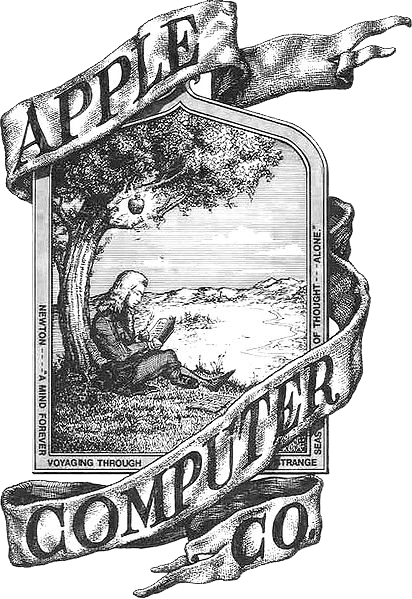
\includegraphics[width=0.5\textwidth]{Apple_first_logo.png}
		\caption{Apple First Logo}
	\end{figure}
	
\section{Body}

\section{Conclusion}

\end{document}
